%\documentclass{article}
\documentclass[tikz,border=5pt]{standalone}
\usepackage{tikz}
\usetikzlibrary{shapes.geometric, arrows, positioning,shapes.misc}
\tikzstyle{startstop} = [rectangle, rounded corners, minimum width=3cm, minimum height=1cm,text centered, draw=black, fill=red!30]
\tikzstyle{io} = [trapezium, trapezium left angle=70, trapezium right angle=110, minimum width=3cm, minimum height=1cm, text centered, draw=black, fill=blue!30]
%\tikzstyle{process} = [rectangle, minimum width=3cm, minimum height=1cm, text centered, draw=black, fill=orange!30]
\tikzstyle{process} = [rectangle, minimum width=3cm, minimum height=1cm, text centered, text width=3cm, draw=black, fill=orange!30]
\tikzstyle{decision} = [diamond, minimum width=3cm, minimum height=1cm, text centered, draw=black, fill=green!30]
\tikzstyle{arrow} = [thick,->,>=stealth]
%Rounded corners only at one side of a TikZ node
\tikzstyle{data} = [fill=gray, rounded rectangle, minimum width=2cm, minimum height=1cm]

\begin{document}
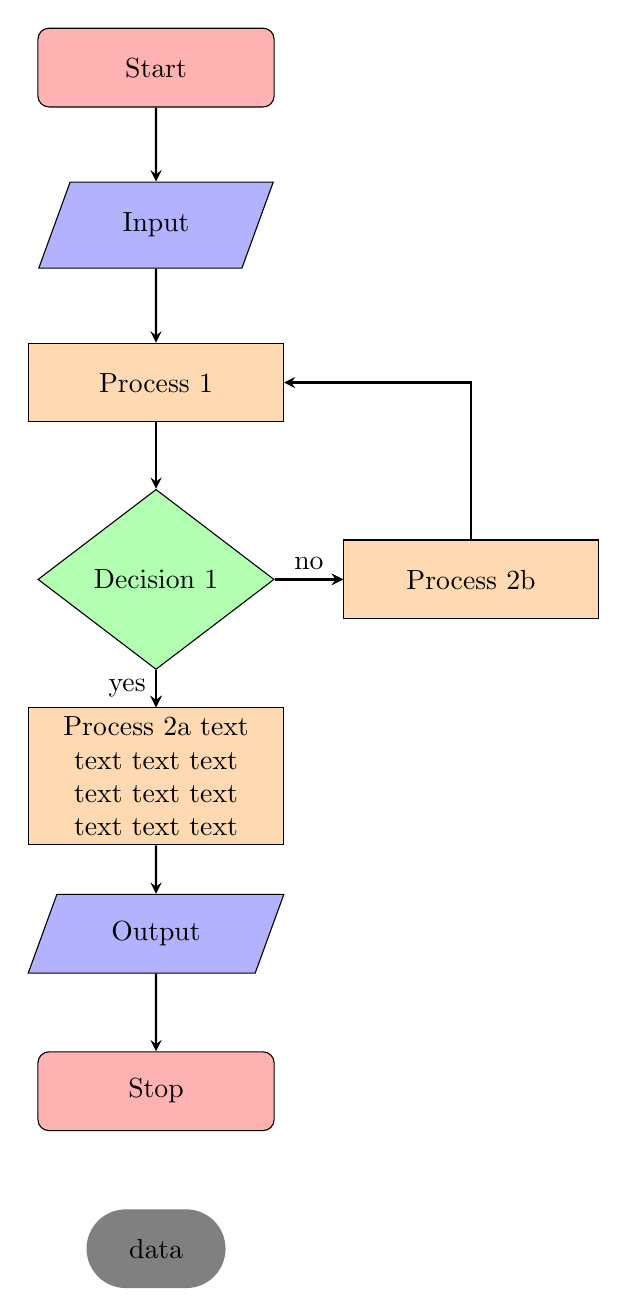
\begin{tikzpicture}[node distance=2cm]

%<TikZ code>
\node (start) [startstop] {Start};
\node (in1) [io, below of=start] {Input};
\node (pro1) [process, below of=in1] {Process 1};
%\node (dec1) [decision, below of=pro1] {Decision 1};
%decision block, being a diamond, is taller than the other blocks. 
%Therefore we can manually adjust its position using the ‘yshift’ variable. 
%If we enter yshift=-0.5cm it will move the decision block 
%vertically down by 0.5cm which should make the gap more regular.
\node (dec1) [decision, below of=pro1, yshift=-0.5cm] {Decision 1};
%\node (pro2a) [process, below of=dec1, yshift=-0.5cm] {Process 2a};
\node (pro2a) [process, below of=dec1, yshift=-0.5cm] {Process 2a text text text text text text text text text text};
\node (pro2b) [process, right of=dec1, xshift=2cm] {Process 2b};
\node (out1) [io, below of=pro2a] {Output};
\node (stop) [startstop, below of=out1] {Stop};
\node (test) [data, below of=stop] {data};

%% draw you chart here

\draw [arrow] (start) -- (in1);
\draw [arrow] (in1) -- (pro1);
\draw [arrow] (pro1) -- (dec1);
\draw [arrow] (dec1) -- (pro2a);
\draw [arrow] (dec1) -- (pro2b);
%\draw [arrow] (dec1) -- node {yes} (pro2a);
%\draw [arrow] (dec1) -- node {no} (pro2b);
\draw [arrow] (dec1) -- node[anchor=east] {yes} (pro2a);
\draw [arrow] (dec1) -- node[anchor=south] {no} (pro2b);
%\draw [arrow] (pro2b) -- (pro1);
\draw [arrow] (pro2a) -- (out1);
\draw [arrow] (out1) -- (stop);
\draw [arrow] (pro2b) |- (pro1);

\end{tikzpicture}


\end{document}
